% !TeX spellcheck = cs_CZ
{\tikzset{external/prefix={tikz/FYZI/}}
 \tikzset{external/figure name/.add={ch24_}{}}
%---------------------------------------------------------------------------------------------------
% file fey1ch27.tex
%---------------------------------------------------------------------------------------------------
%========================= Geometrická optika ======================================================
\chapter{Geometrická optika}\label{fyz:IchapXXVII}
\minitoc

  \section{Úvod}\label{fyz:IchapXXVIIsecI}
    Na několika přístrojích předvedeme aproximaci nazvanou \emph{geometrická optika}. Je to
    nejužitečnější aproximace pro praktickou konstrukci mnoha optických systémů a přístrojů.
    Geometrická optika je buď velmi jednoduchá nebo velmi komplikovaná.
    
    Abychom mohli pokračovat potřebujeme jeden geometrický vztah a to: máme-li trojúhelník s malou
    výškou $h$ a velkou základnou $d$, pak přepona $s$ je delší než základna (viz obr.
    \ref{fyz:fig156}).  
    
    Tedy 
    \begin{equation}\label{FYZ:eq_triangle}
     \Delta \approx \frac{h^2}{2s}.
    \end{equation}
    To je celá geometrie, kterou je třeba znát, aby bylo možné diskutovat vznik obrazů pomocí
    zakřivených ploch.
    
    \begin{figure}[ht!]
      \centering
      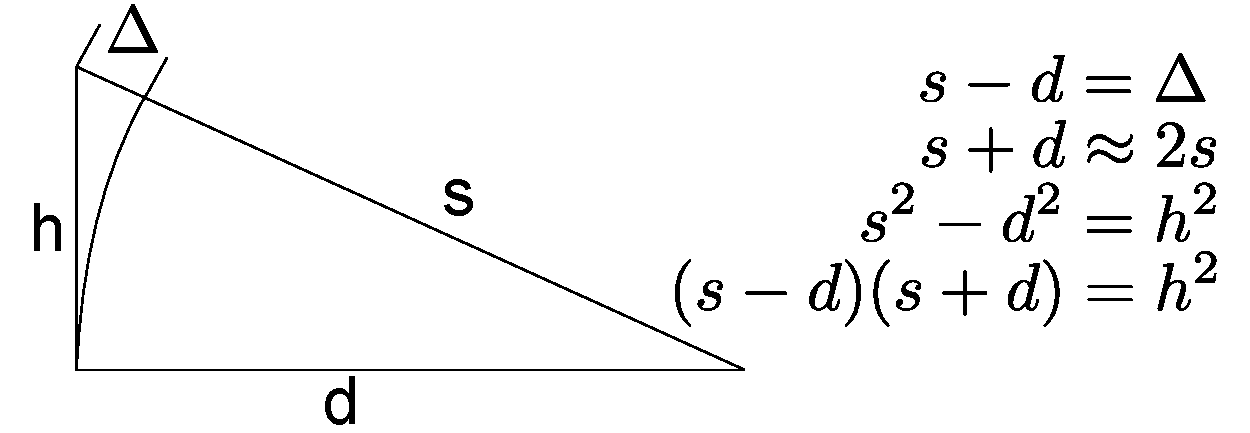
\includegraphics[width=0.6\linewidth]{fyz_fig156.pdf}
      \captionof{figure}{Trojúhelník s malou výškou a velkou základnou
                 \cite[s.~358]{Feynman01}}
      \label{fyz:fig156}  
    \end{figure}

  \section{Ohnisková vzdálenost kulové čočky}\label{fyz:IchapXXVIIsecII}
  \section{Ohnisková vzdálenost čočky}\label{fyz:IchapXXVIIsecIII}
  \section{Zvětšení}\label{fyz:IchapXXVIIsecIV}
  \section{Složené čočky}\label{fyz:IchapXXVIIsecV}
  \section{Aberace}\label{fyz:IchapXXVIIsecVI}
  \section{Rozlišovací schopnost}\label{fyz:IchapXXVIIsecVII}
  \section{Příklady a cvičení}\label{fyz:IchapXXVIIsecVIII}
  
} %tikzset
%~~~~~~~~~~~~~~~~~~~~~~~~~~~~~~~~~~~~~~~~~~~~~~~~~~~~~~~~~~~~~~~~~~~~~~~~~~~~~~~~~~~~~~~~~~~~~~~~~~
\printbibliography[title={Seznam literatury}, heading=subbibliography]
\addcontentsline{toc}{section}{Seznam literatury}